\chapter{Demos clásicas}

\section{Fuego}

\subsection{Investigación inicial}

Una demo que simule un efecto de fuego se podría considerar algo así como el "hola mundo" de la demoscene. Es un ejercicio sencillo con un resultado final bastante espectacular.\\

Tras una búsqueda de información inicial, pude encontrar también dos sitios diferentes en los que se explicaba cómo crear un efecto de fuego.\\ 

En el canal de YouTube de Creature Mann\footnote{\url{https://www.youtube.com/user/kjlg74/featured}} se explica la base teórica para crear un efecto de fuego sencillo\footnote{\url{https://www.youtube.com/watch?v=_SzpMBOp1mE}}. A este vídeo le siguen un par de vídeos de este mismo creador\footnote{\url{https://www.youtube.com/watch?v=iezD8B1ym3w}}\footnote{\url{https://www.youtube.com/watch?v=206TEPBOnLc}} en los que itera sobre el efecto anteriormente creado, añadiendo complejidad (como la posibilidad de controlar la dirección del fuego o trazar un camino que se prende fuego). Por desgracia, los enlaces provistos al código que estos vídeos muestran están caídos, por lo que el código no es accesible. No obstante, la parte argumentablemente más importante, la explicación teórica del efecto, se hace en el primer vídeo.\\

Otra página que ofrece una descripción muy buena del efecto es Lode's Computer Graphics Tutorial\footnote{\url{https://lodev.org/cgtutor/fire.html}}. Esta página sí que aporta código, aunque decidí ignorar la implementación (para evitar que condicionara mi propio desarrollo) y centrarme únicamente en la explicación teórica que se ofrecía, muy similar a la del vídeo anterior aunque más técnica.\\

\subsection{Planteamiento formal}

El fuego es un efecto muy sencillo tanto a nivel teórico como de implementación. Consiste en la convolución de una matriz como la de la figura [\ref{fig:firematrix}] a lo largo de una matriz que tan sólo contiene valores en su fila inferior. Al aplicar esta operación de abajo a arriba, se obtiene un conjunto de valores [\ref{fig:fire_whitegrid}] que al ser asociados a un set concreto de colores [\ref{fig:fire_colouredgrid}], dan una sensación similar al fuego.

\begin{figure}
	\begin{equation}
		\begin{bmatrix}
			0 & 0 & 0 \\
			0 & 0 & 0 \\
			\frac{1}{3} & \frac{1}{3} & \frac{1}{3}
		\end{bmatrix}
	\end{equation}
	\caption{Matriz de convolución para generar efecto de fuego}
	\label{fig:firematrix}
\end{figure}

\begin{figure}[h]
	\centering
	\begin{subfigure}[b]{0.45\textwidth}
		\centering
		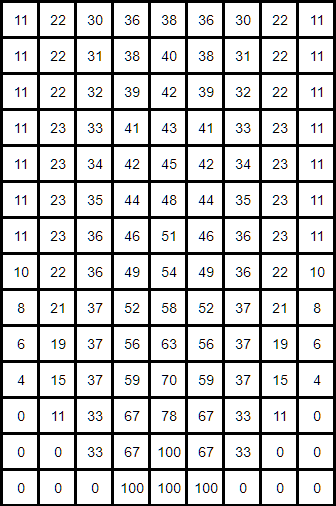
\includegraphics[width=5.09cm]{archivos/fire_whitegrid}
		\caption{Valores resultantes tras convolucionar iterativamente la matriz [\ref{fig:firematrix}] por una matriz de ceros, con valores solo en la fila inferior}
		\label{fig:fire_whitegrid}
	\end{subfigure}
	\begin{subfigure}[b]{0.45\textwidth}
		\centering
		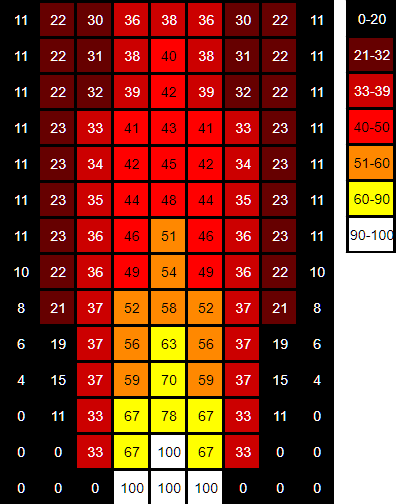
\includegraphics[width=6cm]{archivos/fire_colouredgrid}
		\caption{Efecto resultante de asociar determinados rangos de valores a un set de colores preestablecido}
		\label{fig:fire_colouredgrid}
	\end{subfigure}
\end{figure}


\subsection{Implementación}
\subsection{Refinamiento}
\subsection{Resultado}

\section{Geometría}

\subsection{Investigación inicial}
\subsection{Planteamiento formal}
\subsection{Implementación}
\subsection{Refinamiento}
\subsection{Resultado}

\section{Planos infinitos}

\subsection{Investigación inicial}
\subsection{Planteamiento formal}
\subsection{Implementación}
\subsection{Refinamiento}
\subsection{Resultado}

\section{Plasma}

\subsection{Investigación inicial}
\subsection{Planteamiento formal}
\subsection{Implementación}
\subsection{Refinamiento}
\subsection{Resultado}

\section{RotoZoom}

\subsection{Investigación inicial}
\subsection{Planteamiento formal}
\subsection{Implementación}
\subsection{Refinamiento}
\subsection{Resultado}

\section{Deformaciones de imagen}

\subsection{Investigación inicial}
\subsection{Planteamiento formal}
\subsection{Implementación}
\subsection{Refinamiento}
\subsection{Resultado}

\section{Túnel de puntos}

\subsection{Investigación inicial}
\subsection{Planteamiento formal}
\subsection{Implementación}
\subsection{Refinamiento}
\subsection{Resultado}